\yesmargins
\chapter{Requirements}
\begin{tikzpicture}[overlay,remember picture] 
\node[anchor=south] at ([yshift=5in,xshift=0.85in]current page text area.south){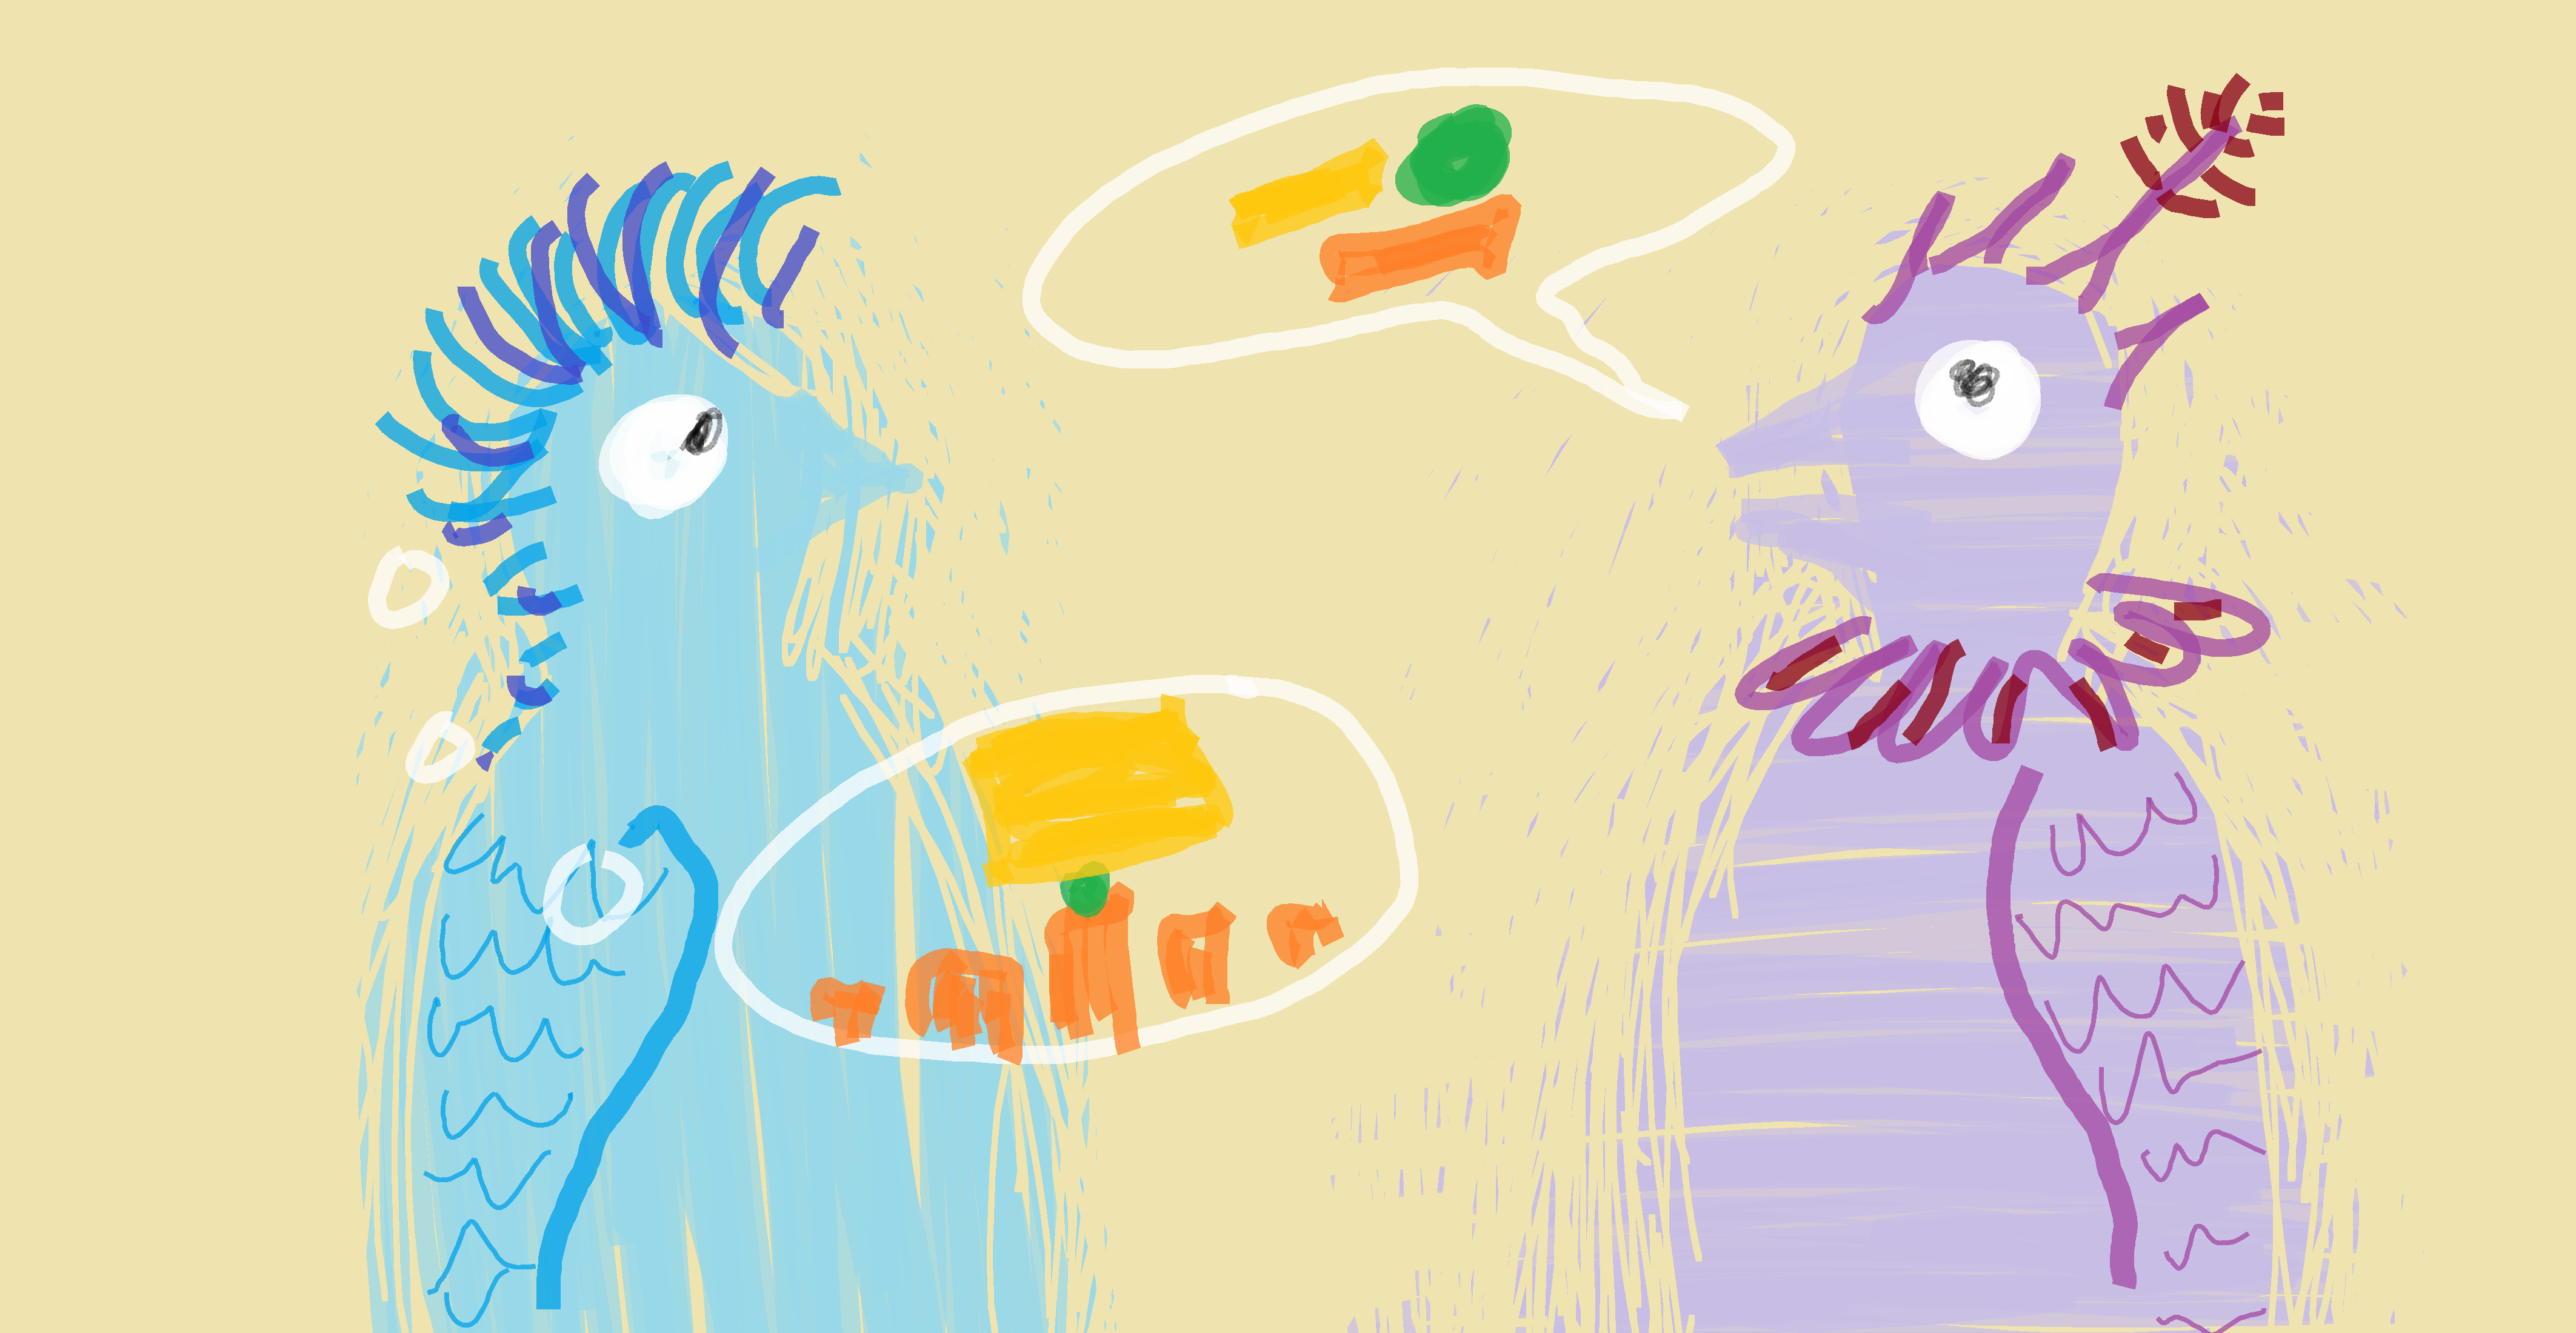
\includegraphics[width=9.5in]{req01}}; 
\end{tikzpicture}\marginpar{ \requirementDef\margindivider}\marginpar{\nonFunctionalRequirementDef\margindivider}\marginpar{\functionalRequirementDef}A software \textbf{requirement}\index{requirements} is a rule the software must conform to: What it must do, how well, and within what constraints or limits.

\section{Types of Requirements}

There are \textbf{two types of requirements}\index{requirements}:

\begin{enumerate}
\item \textbf{Non-functional requirements\index{requirements}\index{non-functional requirements}} specify qualities the software should have (e.g., usable, portable, modular, etc.). They answer the questions, ``How well should the software perform?'' and ``What limits or constraints is the software subject to?'' This chapter includes a discussion of how \textbf{quality attributes}\marginpar{\qualityAttributeDef}\index{quality attributes} can be used in specifying non-functional requirements\index{non-functional requirements}.
\item \textbf{Functional requirements\index{requirements}\index{functional requirements}} specify the desired functionality of software (e.g., if I click the Log In button, the Login page appears). They answer the question, ``What should the software do?'' In this chapter, we'll talk about specifying functional requirements\index{requirements}\index{functional requirements} with user stories\index{user story} and use cases.\marginpar{User stories and use cases are two different methods for specifying functional requirements. As you will see later, one is more formal than the other.}
\end{enumerate}

\begin{center}
\pdftooltip{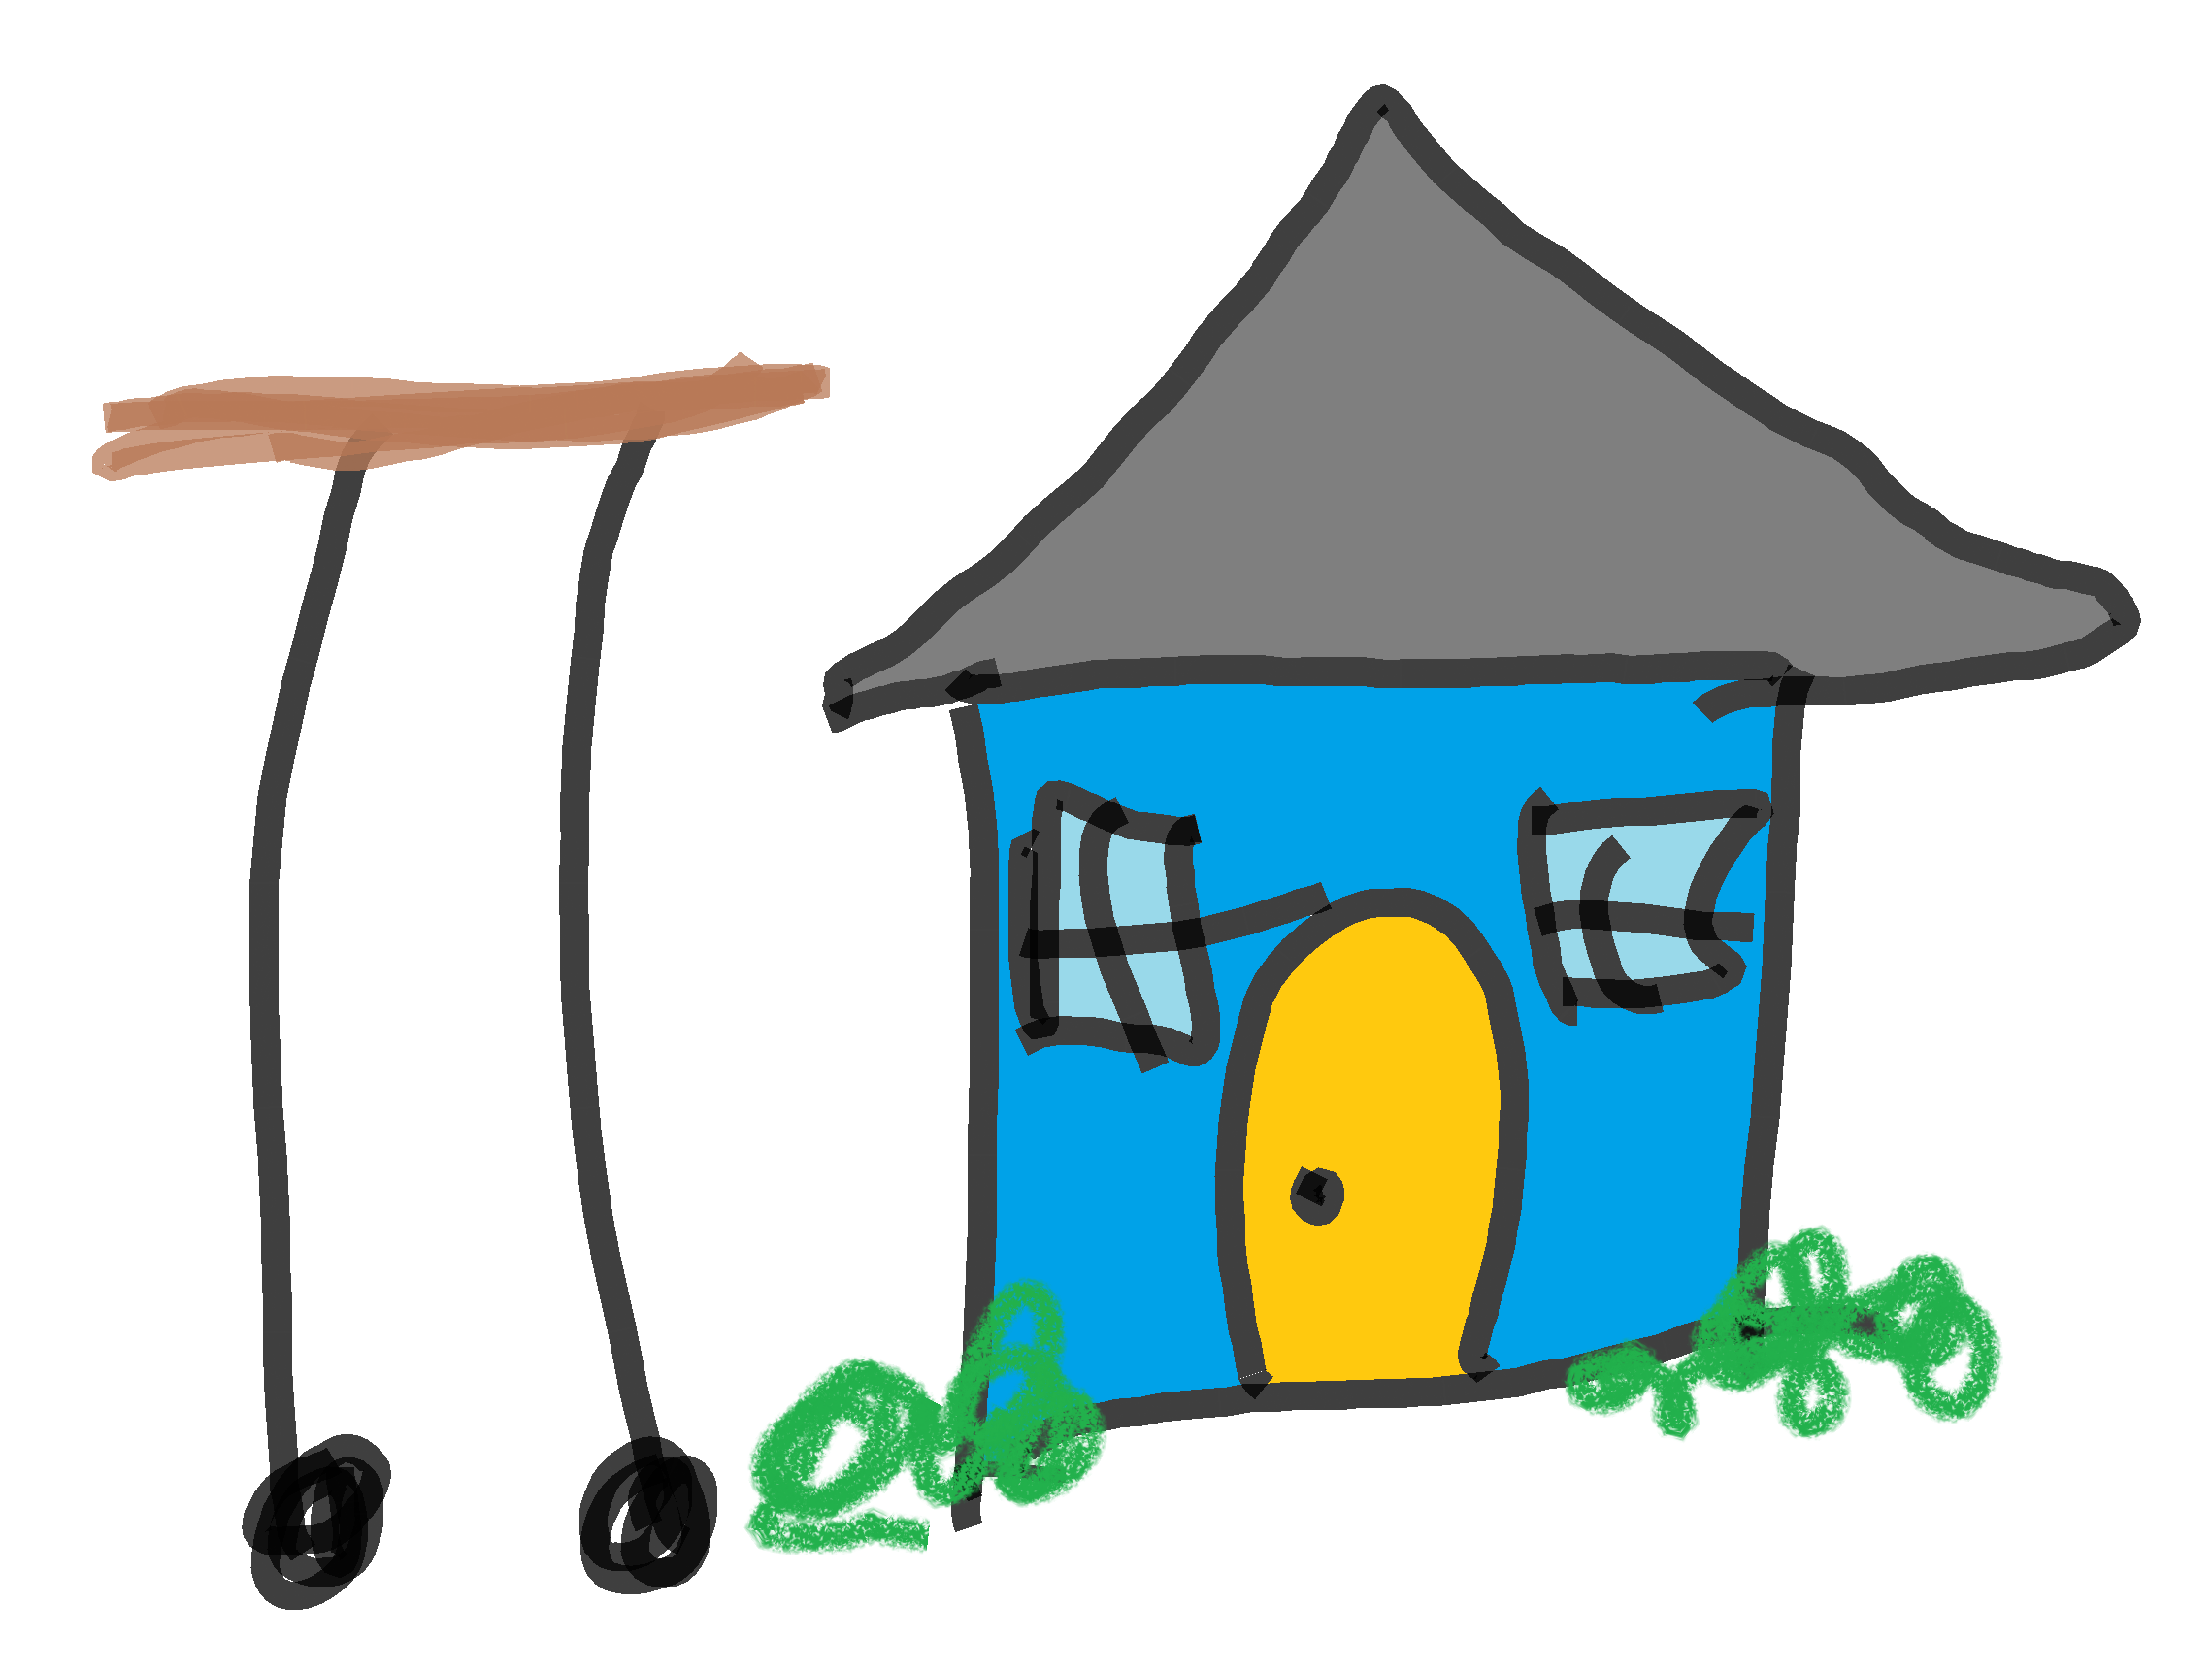
\includegraphics[width=0.5\textwidth]{req02}}{Tall table with only two legs next to a house with a small door.}
\end{center}

\textit{This rolling table fails the non-functional requirement\index{non-functional requirements} of fitting through an average door and the functional requirement\index{functional requirements} of having four legs.}

\section{Why Requirements Matter}

The design\index{design} and implementation\index{implementation} of software should, ideally, follow from the requirements. Here are some ways requirements\index{requirements} are helpful and reasons they are important:\marginpar{Requirements keep the development team on track and working together toward creating what the client (and hopefully the users) want.}

\begin{itemize}
\item When developers aren't given requirements, they \textbf{might prioritize functionality they personally think is important or fun} to implement---but what developers want to implement might not make the project successful.
\item When multiple developers are working on the same code, requirements can \textbf{help them stay in sync} with one another and \textbf{have the same goal}. Without requirements, time, effort, and money can be wasted implementing conflicting code.\marginpar{Requirements can help protect projects from drift and failure.}
\item When requirements\index{requirements} aren't specified, it's easier for project stakeholders\index{stakeholders} (e.g., \textbf{clients}, partners, investors, consultants, management, etc.) to \textbf{influence the project toward satisfying their own} (possibly fleeting) \textbf{wants or needs}. This can result in the project drifting away from what it was originally intended to do---and can lead to project failure.
\item Requirements are \textbf{helpful for communicating} about software with stakeholders\index{stakeholders}, \textbf{keeping track} of everything that needs to get done, and helping you and the client \textbf{decide what really needs to get done} (clients sometimes don't know what they really need).
\end{itemize}\marginpar{\clientDef\margindivider}

\section{What Makes a Good Requirement}

\noindent\textbf{Good requirements have the following characteristics:}\marginpar{Sloppy requirements can be useless or worse.\margindivider}\marginpar{\stakeholderDef}

\spacer
\rowcolors{2}{gray!25}{white}
\noindent\begin{tabular}{p{1in} p{3in}}
\rowcolor{gray!25}
\textbf{Correct} & What they say is right.\\
\textbf{Consistent} & They aren't contradictory of each other.\\
\textbf{Unambiguous} & There is only one way to interpret them.\\
\textbf{Complete} & They cover all that's important.\\
\textbf{Relevant} & They meet a stakeholder need.\\
\textbf{Testable} & There's a way to figure out if they're satisfied.\\
\textbf{Traceable} & It's possible to figure out where they came from.\\
\end{tabular}
\spacer

Requirements that fail to have these characteristics can lead developers to making features of software nobody wants, wasting time and other resources and potentially jeopardizing the project.

\section{Requirements Elicitation}\index{requirements elicitation}

\marginpar{\requirementsElicitationDef}

The process of gathering requirements is called \textbf{requirements elicitation}. Requirements can come from any stakeholder, including clients, managers, users, governments, developers of software your software will integrate with, your development team, and yourself.

\spacer
\noindent\textbf{Three of the most important, distinct, and universal (common across projects) categories of stakeholders:}

\begin{itemize}
\item{\textbf{Clients}\index{clients}: The people who request the software and have most of the authority over its requirements (e.g., because they are paying for it).}
\item{\textbf{Users}\index{users}: The people who will use the software.}
\item{\textbf{Developers}\index{developers}: The people who will make the software, including those who manage the software engineers.}
\end{itemize}

\spacer
\noindent\textbf{Aspects of these stakeholders\index{stakeholders} that can affect the requirements elicitation processes and the software's development and ultimate success:}\\

\begin{itemize}
\item{\marginpar{\tripleConstraintDef\margindivider}\marginpar{\focusGroupDef\margindivider}\marginpar{\usabilityTestingDef\margindivider}\marginpar{\mvpDef\margindivider}\marginpar{\softwareProcessModelDef}\textbf{Clients might not have experience or expertise}. Developers can help fill the gap between what the client wants and what is technically feasible and reasonable (e.g., given time\index{project time}, cost\index{project cost}, and scope\index{scope}, a.k.a. the \textbf{triple constraint}\index{triple constraint}).}\\
\item{\textbf{Clients\index{clients} might not have good ideas}. They may be incorrect about what users will want or will use. Developers sometimes try to guide clients toward better ideas, but developers can also have bad ideas. Methods such as \textbf{focus groups}, \textbf{usability testing}, and releasing a \textbf{minimum viable product} (MVP)\index{minimum viable product (MVP)} can help with figuring out whether users will use (and pay for) the software.}\\
\item{\textbf{Clients might not know what they want}. They might have a rough idea, or they might have an idea that's at odds with their goals. Developers, through requirements elicitation\index{requirements elicitation}, can help clients define their goals clearly and reasonable ways for accomplishing those goals.}\\
\item{\textbf{Users\index{users} might not know what they want or will use}. They may be unaware of their own needs or wants until there's a product in front of them that addresses those needs or wants. Even if 10,000 users tell you, ``I would definitely use an app that does X'', they might be wrong, they might only use the app once, or they might not be willing to pay for the app. MVP can be a good method for figuring out early whether users will be interested enough in the software to use or pay for it.}\\
\item{\textbf{Users\index{users} might want what's bad for them}. You can probably think of multiple examples.}\\
\item{\textbf{Developers\index{developers} have their own tendencies}. They may have technologies and ideas they prefer or feel most comfortable with. For better or worse, they bring their own influences to a project.}\\
\item{\textbf{Clients\index{clients}, users\index{users}, and developers\index{developers} are all humans}. They communicate imperfectly.}\\
\end{itemize}

Deciding what software to make, and doing so successfully, is a complex process influenced by human factors affecting all involved.

So how does one elicit requirements\index{requirements elicitation}? By having conversations or otherwise collecting information from stakeholders\index{stakeholders}. The amount of stakeholder communication can vary by project, project type, the software process model\index{software process model} being used, and other factors.

\section{Non-Functional Requirements}

\marginpar{\nonFunctionalRequirementDef}Non-functional requirements\index{non-functional requirements} describe how well the software needs to perform.

\spacer
\noindent\textbf{Examples of non-functional requirements:}\\

\begin{itemize}
\item Response time should be a few seconds or less in all operating environments.\\
\item The keylogger must be indetectable to 99.999\% of test users.\\
\item The software must be available 24 hours a day, 7 days a week, and must have an uptime of 99.99\%.\\
\end{itemize}

Notice that each requirement\index{requirements} has a \textbf{quantity associated} with it: That makes it testable (a criterion for a good requirement).

\subsection{Quality Attributes}

\marginpar{\qualityAttributeDef}Quality attributes\index{quality attributes} are characteristics of software used to describe how good it is. They can be used in specifying non-functional requirements\index{non-functional requirements}.

\spacer
\noindent\textbf{Examples of quality attributes:}\\

\begin{itemize}
\item \textbf{Reliability\index{reliability}}: How often does function X succeed?
\item \textbf{Efficiency\index{efficiency}}: How many resources does the software need?
\item \textbf{Integrity\index{integrity}}: How frequently does the software have errors that require a restart?
\item \textbf{Memorability\index{memorability}}: How many times must users learn a function before they no longer need documentation? 
\item \textbf{Flexibility\index{flexibility}}: How many ways can the software be used?
\item \textbf{Interoperability\index{interoperability}}: How well can the software integrate with other software?
\item \textbf{Reusability\index{reusability}}: To what extent can the code be used to solve other problems without being modified?\\
\end{itemize}

Each quality attribute\index{quality attributes} can be converted to a scale. For example, the lowest value on a reliability\index{reliability} scale could be ``the function succeeds 0\% of the time'' and 100\% would of course be the opposite pole. Given this scale, we can specify a non-functional requirement\index{non-functional requirements} by defining a performance threshold:\marginpar{A quality attribute\index{quality attributes} is \textbf{not the same as a non-functional requirement}. Rather, quality attributes are good for labelling what a non-functional requirement is about.}

\begin{displayquote}
The function must have high reliability\index{reliability} (succeeds $>$99\% of the time).
\end{displayquote}

When you select quality attributes\index{quality attributes} for your software, you are prioritizing what qualities matter most to you / your team / the project. Ideally, your team would keep these quality attributes (and the corresponding non-functional requirements\index{non-functional requirements}) in mind for the duration of the project; If the software is not meeting the non-functional requirements, either the software or the threshold of acceptability needs to change.

\section{Functional Requirements}

\marginpar{\functionalRequirementDef}

\spacer
\noindent\textbf{Example of a functional requirement:}
\begin{displayquote}
When a user clicks the ``register'' button, their information is added to the database and the user is shown a ``thank you for registering'' screen.
\end{displayquote}

\subsection{User Stories}

\textbf{User stories}\index{user story} are a method for specifying functional requirements. They describe a small piece of the software's functionality in a simple and easy to read sentence. They are written in plain English so that non-technical people (e.g., users, clients\index{clients}, other stakeholders\index{stakeholders}) can understand them.

\marginpar{\userStoryDef}\index{user story}User stories have a title and are commonly written using this format:
\begin{displayquote}
As a $\langle$ROLE$\rangle$, I want $\langle$SOME FUNCTIONALITY$\rangle$ so that I get $\langle$SOME BENEFIT$\rangle$.
\end{displayquote}

These short sentences can be written on 3x5'' index cards and then stuck on a wall or whiteboard. They can also be typed into task and project management\index{project management} systems (e.g., Jira\index{Jira}, Asana\index{Asana}, etc.).

\spacer
\noindent\textbf{Examples of what user story cards can look like:}

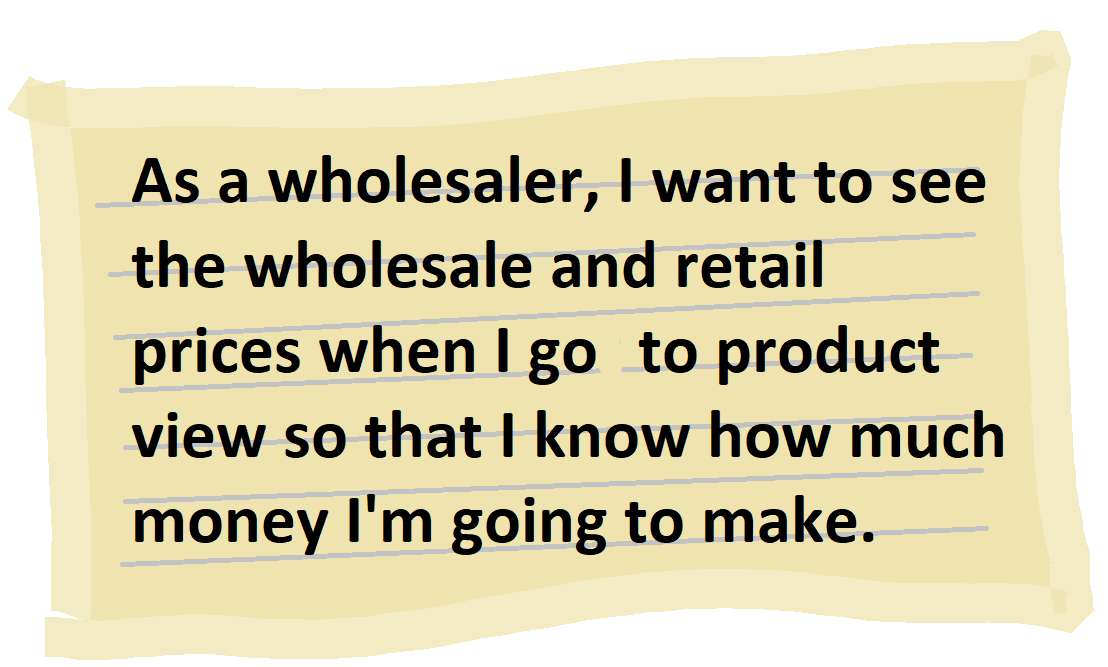
\includegraphics[width=0.8\textwidth]{req04}

\marginpar{More examples of user stories: \url{https://tinyurl.com/user-story-examples}\\
\url{https://twitter.com/shituserstory}}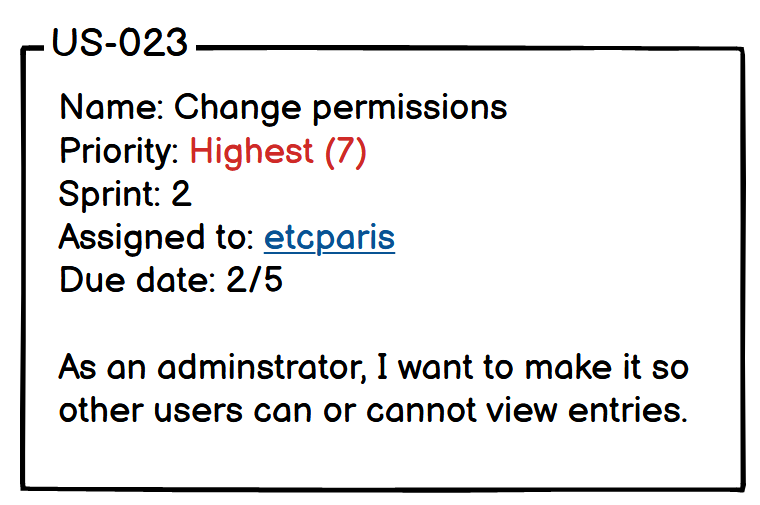
\includegraphics[width=0.8\textwidth]{req05}

Anyone on the team---or any project stakeholder\index{stakeholders}---might come up with user stories. Once the user stories are initially defined, they can be used to start a conversation with the client and others on the team. Clients\index{clients} can guide you on setting priorities for user stories. This conversation is also a good time to get more details about the user stories\index{user story}, which should be added to the card.

\spacer
\marginpar{\investDef}\noindent\textbf{Characteristics of good user stories (INVEST)\index{INVEST}:}

\spacer
\rowcolors{2}{gray!25}{white}
\noindent\begin{tabular}{p{0.25in} p{4in}}
\rowcolor{gray!25}
I & \textbf{Independent}: Doesn't depend on other user stories.\\
N & \textbf{Negotiable}: Can be changed during development.\\
V & \textbf{Valuable}: Fulfills a user need.\\
E & \textbf{Estimable}: Can be given a time estimate.\\
S & \textbf{Small}: Can fit into a single development period (e.g., a 2-week Sprint)\\
T & \textbf{Testable}: Possible to determine it's done.\\
\end{tabular}
\spacer

There is some overlap between INVEST\index{INVEST} and the general characteristics of good requirements mentioned earlier in this chapter.

\marginpar{\acceptanceCriterionDef\index{acceptance criteria}\margindivider}\marginpar{\dodDef}\index{definition of done (DoD)}\index{DoD (definition of done)}How do you know when you are done with a user story? This is negotiated with the client and added to the user story as acceptance criteria. Acceptance criteria\index{acceptance criteria} say what must be true about the functionality specified by the user story in order for the user story to be considered done (i.e., establishing the \textbf{Definition of Done}\index{definition of done (DoD)} for the user story\index{user story}).

\spacer
\noindent\textbf{Example acceptance criterion:}

\begin{displayquote}
\textbf{Given} the user is playing a video file \textbf{and} their operating system is Windows, \textbf{when} they do the Ctrl-T keyboard shortcut \textbf{then} they will see the ``Go to Time'' screen \textbf{and} the video will pause.
\end{displayquote}

There are bolded words in that example because its using a common format \parencite{agilealliance} for acceptance criteria\index{acceptance criteria}:

\begin{displayquote}
Given \ldots when \ldots then \ldots
\end{displayquote}

The ``and'''s are optional parts of the format. Ideally, acceptance criteria\index{acceptance criteria} testing can be automated.

\spacer
\noindent\textbf{Example pseudocode for testing acceptance criteria\index{acceptance criteria}:}

\lstinputlisting[language=Python]{code/req-acceptance-test.py}

\subsection{Use Cases}

\marginpar{\useCaseDef}\textbf{Use cases} are a more formal method of specifying functional requirements\index{functional requirements}. They are structured descriptions of what a system is required to do when a user interacts with it.

Use cases are not specific to a particular software process model\index{software process model} (e.g., Agile\index{agile}, Waterfall\index{waterfall (software process model)}, Spiral\index{spiral (software process model)}) or environment. Instead, like much of what you will encounter in this book, they are a well-known method software teams can choose to use (and many do), or not.

\spacer
\marginpar{More examples of use cases\index{use case}: \url{https://tinyurl.com/use-case-examples}}\textbf{Example of a use case:}
\spacer

\begin{itemize}
\item{\textbf{Name}: Generate list of recovered patients}
\item{\textbf{Actor}: Clinician}
\item{
\textbf{Flow}:
\begin{enumerate}
\item Clinican authenticates using smart card
\item Software confirms credentials and access permissions for specific machine
\item Software logs access
\item Software displays patient search
\item Clinician selects ``Advanced Patient Search''
\item Software confirms user access permissions for advanced search page
\item Clinician selects ailment and patient status
\item Clinician executes search using ``Search'' button
\item Software returns results
\item Software logs query
\end{enumerate}
}
\end{itemize}

\subsubsection*{Required Parts of a Use Case}

What every valid use case\index{use case} has:

\begin{itemize}
\item \textbf{Name}: A short title for the use case that often starts with a verb (e.g., Schedule weekly wellness check). Briefly states the user objective the use case will be describing.
\item \textbf{Actors}: The user or users (human / non-human / computer) that are interacting with the software (e.g., Medical staff)
\item \textbf{Flow of events} (a.k.a. ``basic course of action'' or ``success scenario''): Sequence of actions describing the interaction between the actor and the software.
\end{itemize}

Sometimes, the actor is implied through the flow of events (e.g., Shopper selects the calendar icon). Other times, the actor is stated separately from the flow of events (e.g., Actor: Shopper).

\marginpar{The correct amount of detail to give a use case is the minimum amount to adequately describe what you're trying to communicate.}\subsubsection*{Additional Parts of a Use Case}

Sometimes included in use cases\index{use case}:\\

\begin{itemize}
\item \textbf{Identifier\index{identifiers (in use cases)}}: A unique way of referring to the use case (e.g., UC-002)
\item \textbf{Pre-conditions\index{pre-conditions (in use cases)}}: What must be true before the flow (e.g., The shopper has added at least one product to their shopping cart.)
\item \textbf{Post-conditions\index{post-conditions (in use cases)}}: What must be true after the flow (e.g., The shopper received an order confirmation email.)
\item \textbf{Business relevance\index{business relevance (in use cases)}}: Justification for why the use case exists
\item \textbf{Dependencies\index{dependencies (in use cases)}}: Other use cases the use case relies on. This unique identifier is handy for this part.
\item \textbf{Extensions\index{extensions (in use cases)}}: Contingencies, alternate routes, and branches to other use cases
\item \textbf{Priorities\index{priorities (in use cases)}}: The importance of the use case
\item \textbf{Non-functional requirements\index{non-functional requirements}}: How well the software must perform during the flow
\end{itemize}

\section{Requirements Specification}

\marginpar{\requirementsSpecificationDef}The process of writing down requirements is called \textbf{requirements specification}. Used as a noun, requirements specification refers to the document that contains the requirements. That document is also called an \textbf{SRS} (Software Requirements Specification)\index{software requirements specification (SRS)}. The best way to understand what an SRS looks like is to look at some.

\spacer
\noindent\textbf{Freely available SRS\index{software requirements specification (SRS)} examples (including some for open source software):}
\spacer

\begin{itemize}
    \item \marginpar{\srsDef\margindivider}\marginpar{Another type of software document, which sometimes gets confused with an SRS, is a Software Design Document (SDD)\index{software design document (SDD)}. If the SRS is what the software \textit{should} do, the SDD is what the software \textit{is}. However, there is often overlap between the two.}\textbf{SRS for apps and a data repository for distributing manufacturing data}: \fullcite{hedberg17}\\
    \item \textbf{SRS for data system that assesses conservation practices}: \fullcite{datasystemteam}\\
    \item \textbf{SRS for an app that splits and merges PDFs}: \fullcite{spyridonos10}\\
    \item \textbf{SRS for software that processes EEG data}: \fullcite{iniria}\\
    \item \textbf{SRS for library software}: \fullcite{eaker06}
\end{itemize}

\nomargins

\section{Conclusion}
Gathering and writing down requirements for a project can help with keeping the project on track and communicating about the project to others. Doing requirements well can save a project from failing.

\section{Additional Resources}

\begin{description}
\item \fullcite{agilealliance}
\item \fullcite{atkinson99}
\item \fullcite{barnum20}
\item \fullcite{cockburn01}
\item \fullcite{cohn}
\item \fullcite{fowler04}
\item \fullcite{odimegwu00}
\item \fullcite{olsen15}
\item \fullcite{parsons03}
\item \fullcite{wake}
\end{description}